\documentclass{article}

\usepackage[catalan]{babel}
\usepackage[utf8]{inputenc}
\usepackage[T1]{fontenc}
\usepackage{hyperref}
\hypersetup{
    colorlinks=true,
    linkcolor=blue,
    filecolor=magenta,      
    urlcolor=cyan
}


\usepackage{titlesec}

\titleformat{\section}
{\LARGE\bfseries}
{\thesection. }
{0em}
{}[\titlerule]


\usepackage[margin=1.2in]{geometry}

\titleformat{\subsubsection}[runin]
{\bfseries}
{}
{0em}
{}



\title{\textbf{Projecte de llenguatge de marques - CocktailDB}}
\author{Nil Jimeno, Bernat Brucet}

\begin{document}
\maketitle


% car\`acters en \k{C}\'atal\`a


% Normes del repositori:
% - modificar nomes als arxius corresponents importats per \input
% - mantenir una llargada adequada per les linies (no mes de 90 caracters per linia)

% Caracters en catala:
% - \k{c} c trencada
% - \'e accent tancat
% - \`e accent obert
% - \lgem ela ageminada
% No es necessari escriure els caracters aixi, ja que
% es poden escriure els caracters amb accent tambe.


% Text va en aquests arxius:

\section{Justificaci\'o del projecte}
El nostre projecte s'ha fet amb la intenci\'o de
posar en pr\`actica coneixements relacionats amb Python,
per entendre millor la ll\`ogica del llenguatge de programaci\'o
i aprendre i posar en pr\`actica diferents llibreries.
A part de l'inter\`es personal,
est\`a centrat principalment en aprendre tant
Python com a llenguatge de programaci\'o com l'\'us i interacci\'o de llibreries,
no t\'e cap objectiu m\'es enll\`a del coneixement obtingut.


\subsection{Ll\'ogica abans d'abstracci\'o}
El projecte que hem fet est\`a centrat en la llibreria Pyxel.
Un dels punts que la distingeix per sobre d'altres llibreries, com Pygame,
\'es la poca abstracci\'o que utilitza.
D'aquesta manera, el programa est\`a molt m\'es centrat en la ll\`ogica
del programa i l'\'us d'estructures apropiades per posar-lo en pr\`actica.

Encara que tamb\'e hem fet \'us d'altres llibreries,
la base del projecte es basa molt m\'es en el llenguatge en si que
no pas en funcions de llibreries espec\'ifiques,
aix\'i els coneixements obtinguts no son tan situacionals.


\subsection{Llibreries}
Encara que pyxel no se centra en l'\'us de llibreries externes,
\'es important aprendre a utilitzar-les
perque python est\`a molt centrat en el seu \'us.

\subsubsection{Pyxel}
\'Es la llibreria principal.
S'encarrega de controlar que el programa s'executi en bucle de manera controlada,
crear la finestra de l'aplicaci\'o i mostrar gr\`afics per pantalla.

Encara que sigui per python, la llibreria t\'e un rendiment acceptable
perque ha estat programada en Rust.

\subsubsection{Sqlite3}
\'Es un software d'administrador de bases de dades relacionals a nivell local,
per la qual cosa s'utilitza soving en aplicacions. El programa est\`a escrit en C.
S'encarrega d'administrar algunes dades.

\subsubsection{Flask}
Framework simple fet en python, per projectes poc professionals/tests.
S'encarrega de mostrar una p\`agina amb les puntuacions m\`aximes.


\section{Arquitectura del programa}

\subsubsection{Models}
A la carpeta Models es guarden les classes amb els atributs que es reben de l'api.

\subsubsection{Controllers}
\'Es on es guarda l'arxiu cs que manega les trucades a la web i fa les trucades a la api.
Per fer una trucada a l'api,
guarda l'informaci\'o rebuda a una classe (definida a Models)
i a continuaci\'o obre la vista corresponent (definida a Views).

\subsubsection{Views}
\'Es la carpeta a on es guarden les p\`agines en format cshtml.
Es divideix en dues subcarpetes: home, a on es guarden les p\`agines,
i shared, a on es guarda el layout compartit (que es repeteix a totes les p\`agines).

\subsubsection{wwwroot}
\'Es a on es guarden els assets de la web,
incluint el css, la font i la imatge del fons.


\section{Explicaci\'o del codi}

\subsection{HomeController}
El fitxer HomeController.cs \'es l'encarregat de manegar la web.
T\'e una funci\'o per cada p\`agina`,
que prepara la vista d'aquesta i mostra l'html resultant al client.
Dep\`en de la funci\'o executada, carrega una vista o una altra,
que t\'e el mateix nom que la funci\'o.


\subsection{Trucades a la api}
Per aconseguir els valors per mostrar a la p\`agina,
primer es fa una trucada a l'api des de HomeController.cs
(aquesta dep\`en de la p\`agina que est\`a carregant i l'argument que ha rebut).

\begin{figure}[!h]
	\centering
	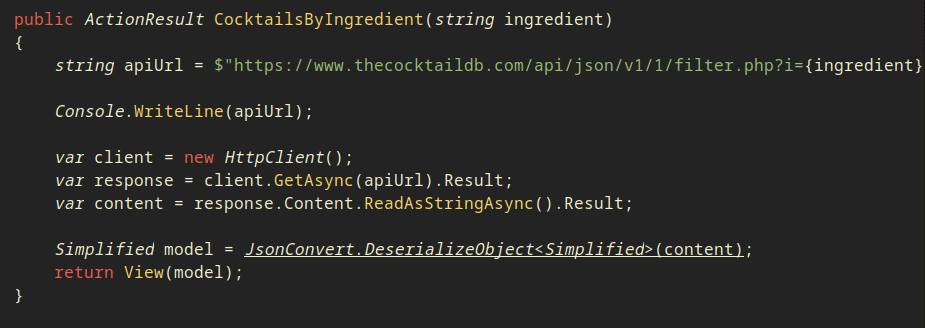
\includegraphics[width=0.8\columnwidth]{homecontroller-ex.png}
	\caption{Exemple de funci\'o a HomeController.cs}
\end{figure}

Els resultats de la trucada s\'on rebuts en format JSON,
que es transforma utilitzant Newtonsoft per guardar-se en la variable model,
que \'es una inst\`ancia d'una classe amb els par\`ametres que es volen mostrar
i s'utilitza com a argument al carregar la vista.
En el nostre cas, les classes s\'on llistes amb informaci\'o sobre
les begudes que es volen mostrar.

\begin{figure}[!h]
	\centering
	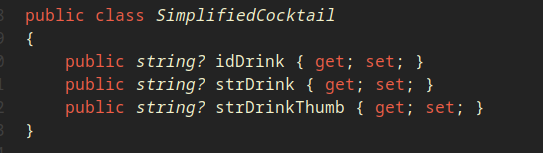
\includegraphics[width=0.8\columnwidth]{simplifiedcocktail.png}
	\caption{Exemple de classe a Cocktail.cs}
\end{figure}


\subsection{Vistes}
Per carregar la vista,
primer s'executen tamb\'e els arxius \_ViewStart.cs i \_ViewImport.cs
per carregar els layouts corresponents i importar els m\`oduls necessaris.

Les vistes s\'on l'html rebut per part del controlador,
que \'es el que es mostra a la pantalla del client.
Aquests es fan a partir dels fitxers cshtml,
que ajunten html amb funcions de C\# i ASP.

Algunes d'aquestes funcions utilitzades s\'on el foreach,
que repeteix un codi html per cada beguda que es vulgui mostrar,
o un if, per comprovar condicions.
Tamb\'e s'utilitzen variables per mostrar par\`ametres a l'html,
com ara la informaci\'o de les begudes mostrades
(incluint t\'itol, descripci\'o, imatge...).

\begin{figure}[!h]
	\centering
	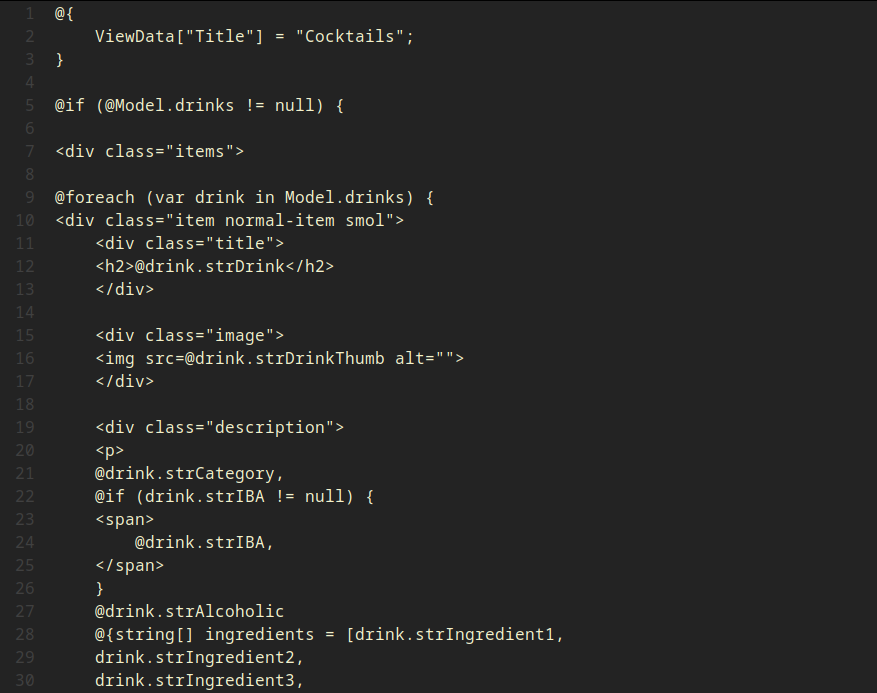
\includegraphics[width=0.8\columnwidth]{cshtml-ex.png}
	\caption{Exemple de cshtml a Cocktails.cshtml}
\end{figure}

Els fitxers de la carpeta home utilitzen comparteixen el codi del layout,
que s'afegeix autom\`aticament a totes les vistes.
Aquest cont\'e configuracions del head, el t\'itol, el navbar i la barra de busca.
\'Es un fitxer compartit per no haver de repetir aquella porci\'o de codi a cada cshtml.

\begin{figure}[!h]
	\centering
	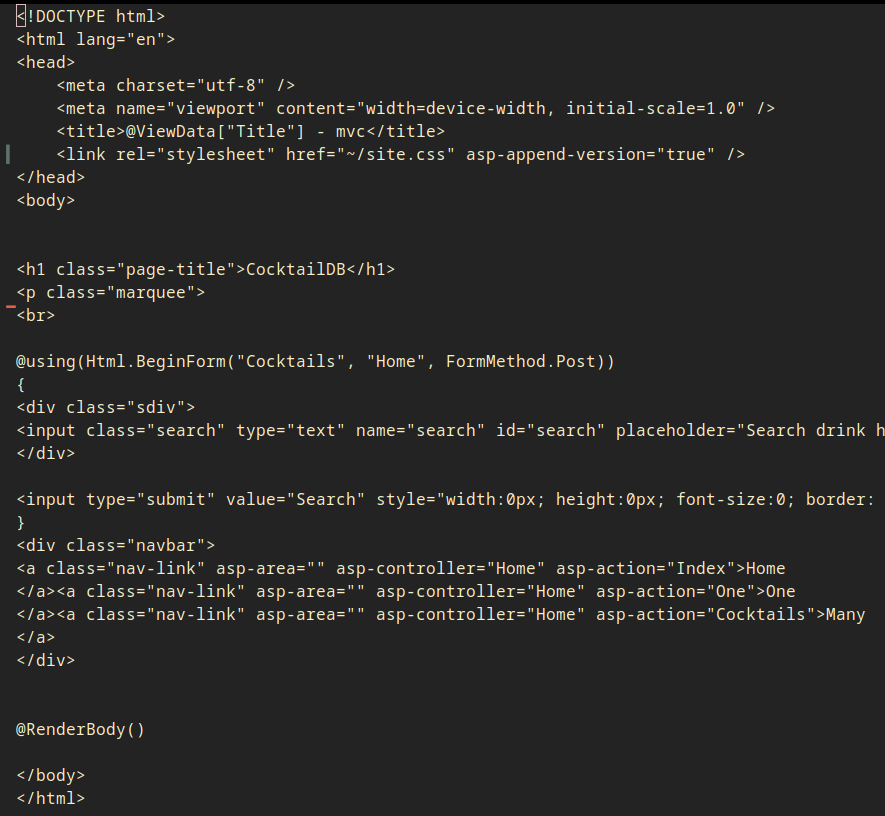
\includegraphics[width=0.8\columnwidth]{cshtml-layout-cut.png}
	\caption{\_Layout.cshtml (tallat)}
\end{figure}

\subsection{Links}
Per anar de p\`agina en p\`agina,
s'utilitzen links amb par\`ametres especials (de cshtml)
que truquen a altres funcions de HomeController.
Per cada funci\'o, es carrega la vista amb aquest mateix nom.
En cas de que requereixin m\'es informaci\'o,
com ara els valors que es volen buscar (com a argument),
s'utilitza asp-target per canviar-los.

D'una manera similar funciona el formulari,
al qual se l'ha d'especificar a quina funci\'o est\`a trucant,
i aquest retornar\'a els valors del formulari en forma d'argument.
Els formularis s\'on utilitzats per fer funcionar la barra de busca.

\section{Possibles millores}

Ens faltaria millorar que quan no trobi una API, no es peti la pàgina web.

\pagebreak



\end{document}
